\phantomsection
\part*{ADN}% -capitulo de string matching con ejemplos ilustrativos propios
% \addcontentsline{toc}{part}{String Matching}

\phantomsection
\section*{Importancia del String Matching con el ADN}
\addcontentsline{toc}{section}{Importancia del String Matching con el ADN}

\quad El Ácido desoxirribonucleico o ADN es un ácido nucleico compuesto de 4 nucleótidos, estos son la adenina (A), timina (T), guanina (G) y citosina (C), además de estos 4 nucleótidos, existe un 5 que es el uracilo (U), pero este se encuentra en el ARN reemplazando a la timina (T). Este contiene las instrucciones y la información genética usadas en el desarrollo y funcionamiento de todo ser vivo, incluyendo algunos virus, además, es el responsable de la herencia genética, como el color de ojos, el color de piel, el cabello y todo tipo de cosas que podemos heredar de nuestros padres o antepasados, sin embargo, también es responsable de heredar ciertas enfermedades genéticas, como por ejemplo, la fibrosis quística, la hemofilia, la enfermedad de Huntington, etc. \\

\quad Para efectos de esta investigación, hemos decidido utilizar la enfermedad de Huntington como ejemplo de string matching en una cadena de ADN. \\

\quad La enfermedad de Huntington es una enfermedad hereditaria que da la instrucción al cuerpo de producir una proteína llamada Huntingtina(HTT). Aunque se desconoce la función de dicha proteína, se cree que juega un papel importante en las neuronas. Esta enfermedad es provocada por una mutación en un segmento del ADN conocido como una repetición del trinucleótido CAG (citosina, adenina y guanina). Este segmento CAG normalmente se repite de 10 a 35 veces en personas sanas, sin embargo, en personas con la enfermedad de Huntington, dicho segmento se repite de 36 a as de 120 veces. \\

Como se puede ver en la siguiente imagen: 
\begin{figure} [H]
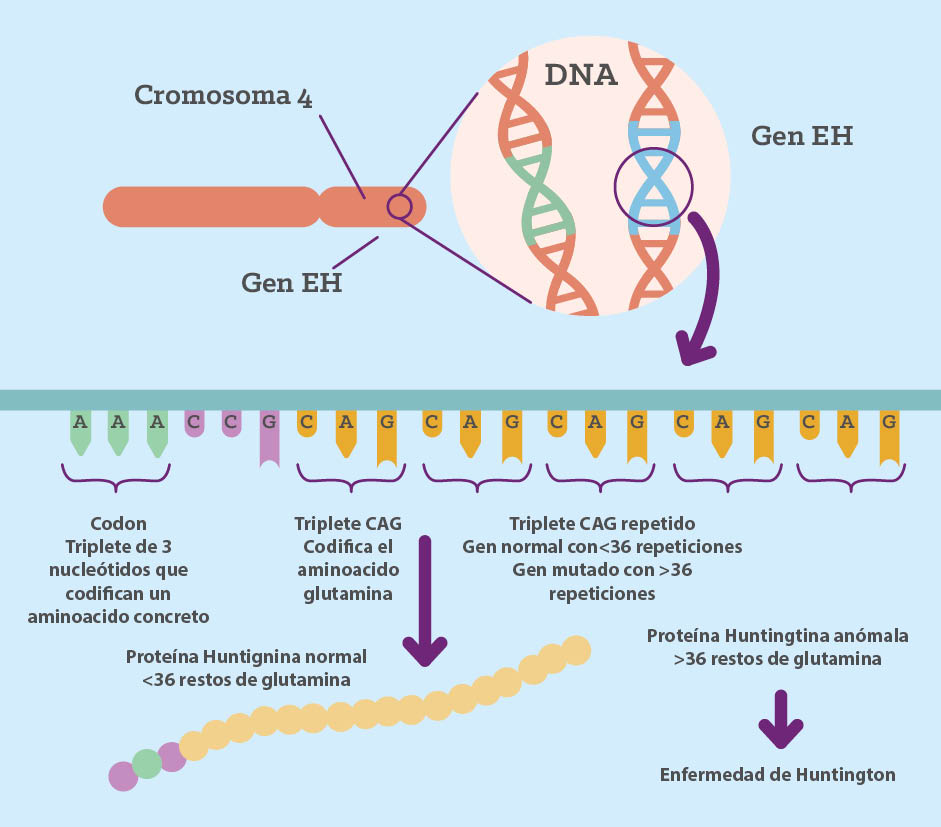
\includegraphics[width=1.0\textwidth]{causas-enfermedad-huntington.jpg}
\caption{Causes de Huntington}
\label{fig:Hunttington}
\end{figure}


\quad Para efectos del string matching, vamos a comprobar cuantas veces se repite  el segmento CAG en la cadena de ADN para comprobar si una persona padece de esta enfermedad.

% https://biolinksperu.com/blog/enfermedades-hereditarias-comunes/
% https://rochepacientes.es/enfermedad-huntington/causas.html